\documentclass[12pt,a4paper]{article}

\usepackage{fullpage}

\usepackage{amsmath, amssymb, amsthm}
\usepackage{babel}[English]
\usepackage{graphicx}
\usepackage{subcaption}
\usepackage{hyperref}
\usepackage{subfiles}
\usepackage[]{algorithm2e}

\usepackage{mathpazo}
\linespread{1.05}

\title{Implementation of a finite difference 1st order upwind scheme to solve the one-dimensional ideal hydrodynamic equations}
\date{\small{\today}}
\author{\normalsize{Fleur Seuren\\ \normalsize{Assignment 1: Computational Methods  Astrophysical Applications}}}

\begin{document}
\maketitle

\section{Introduction}
In this report the one-dimensional hydrodynamic equations will be numerically solved using a finite difference 1st order upwind scheme. The implementation will be checked with two test cases. First, the sod shock problem, where the initial state has a discontinuity and second the isothermal acoustic wave, where the initial conditions are smooth. For the sod shock problem we will perform a convergence analysis. 

\section{Analytic investigation}
The ideal hydrodynamic equations in one dimension are conservation laws for $\rho$, the mass density, $\rho v$, momentum and $e$ total energy. They can be written in matrix form as:
\begin{align}
\partial_{t}\left(\textbf{U}\right) + \partial_{x}\textbf{F}\left(\textbf{U}\right) = 0 \\
\partial_{t}\begin{pmatrix} \rho \\
\rho v \\
e
\end{pmatrix}
+
\partial_{x}\begin{pmatrix} \rho v \\
\rho v^{2} + P \\
\left((e + P) v\right)
\end{pmatrix} = 0. \label{cons_1D}
\end{align}

Equation \eqref{cons_1D} can be rewritten in the form $\partial_t \textbf{U} + \textbf{A}\left(\textbf{U}\right)\partial_x \textbf{U}$, where $\textbf{A}$ is the Jacobian of the flux-matrix: 
\begin{align}
\textbf{A}\left(\textbf{U}\right) = \frac{\partial \textbf{F}}{\partial \textbf{U}} = 
\begin{pmatrix}
0 & 1 & 0 \\
- \left(\frac{3-\gamma}{2}\right)v^{2} & \left(3 - \gamma\right)v & \gamma - 1 \\
- \gamma \frac{v e}{\rho} + \left(\gamma - 1\right)v^{3} & \gamma \frac{ e}{\rho} - \frac{3}{2}\left(\gamma -1 \right)\rho v^{2} & \gamma\frac{\rho v}{e}
\end{pmatrix}. \label{A}
\end{align}

This equation can be solved numerically by diagonalizing this Jacobian, for which we need to compute the eigenvalues and eigenvectors of matrix $\textbf{A}$. 

The easiest way to find the eigenvalues is to compute them using a similar matrix, namely the matrix we obtain by changing the conservative variables, $\rho$, $\rho v$ and $e$ to the primitive variables $\rho$, $v$ and $P$. Because we are working with the ideal hydrodynamic equations $e = \frac{\rho v^{2}}{2} + \frac{p}{\gamma}$ and we find:
\begin{align*}
\partial_{t}\begin{pmatrix} \rho \\
v \\
P
\end{pmatrix}
+
\begin{pmatrix}
v & \rho & 0 \\
0 & v & \frac{1}{\rho} \\
0 & P \gamma & v
\end{pmatrix}
\partial_{x}\begin{pmatrix} \rho \\
v \\
P\right)
\end{pmatrix} = 0. \label{prim_1D}
\end{align}

From the matrix in \eqref{prim_1D} we compute the eigenvalues as follows:
\begin{align*}
\lambda_1 &= v - \sqrt{\frac{P \gamma}{\rho}} = v - c_s \\
\lambda_2 &= v \\
\lambda_3 &= v + \sqrt{\frac{P \gamma}{\rho}} = v + c_s
\end{align*}
where $c_s = \sqrt{\frac{P \gamma}{\rho}}$ is the local speed of sound. 

Now the eigenvectors can be calculated as $\textbf{A}(\textbf{U})E_i = \lambda_i E_i$:
\begin{align*}
E_1 = \begin{pmatrix}
1 \\
v - c_s \\
\frac{v^{2}}{2} - v c_s + \frac{{c_s}^{2}}{\gamma -1} 
\end{pmatrix}, \ 
E_2 = \begin{pmatrix}
2 \\
v \\
\frac{v^{2}}{2}
\end{pmatrix}, \ 
E_3 = \begin{pmatrix}
1 \\
v + c_s \\
\frac{v^{2}}{2} + v c_s + \frac{{c_s}^{2}}{\gamma -1} 
\end{pmatrix}.
\end{align*}

\section{Numerical implementation}
The hydrodynamic equations \eqref{cons_1D} will as stated in the introduction be solved by a first order upwind method. Therefore we define the conservative variables on a mesh discretized in space and time with points $U^{n}_{i}$ (where $i$ denotes the spatial location and $n$ the temporal location) and use a given initial condition at $n = 0$.

Because we are using the first order upwind method the values at the points $U_i^{n}$ will be advanced in time using the following scheme:
\begin{align}
\left\{\begin{matrix}
\frac{U_i^{n+1} - U_i^{n}}{\Delta t} = - \frac{\left({\lambda}_i^{n}U_i^{n} - {\lambda}_{i-1}^{n} U_{i-1}^{n}\right)}{\Delta x} & & {\lambda}_i^{n} > 0 \\
\frac{U_i^{n+1} - U_i^{n}}{\Delta t} = - \frac{\left({\lambda}_{i+1}^{n}U_{i+1}^{n} - {\lambda}_{i}^{n} U_{i}^{n}\right)}{\Delta x} & & {\lambda}_i^{n} < 0 \\
\frac{U_i^{n+1} - U_i^{n}}{\Delta t} = 0 & & {\lambda}_i^{n} = 0
\end{matrix}.
\end{align}
where $\lambda_{i}^{n}$ is the wave-speed at $x_i$ on time $n$. 

The eigenvalues of $\textbf{A}$ are wave-speeds in the following set of independent quasi-linear advection equations where $V = K^{-1}U$ and $K^{-1}$ the inverse eigenvector matrix. 
\begin{align}
\left\{ \begin{matrix}
\partial_t V_1 +  \lambda_1 \partial_x V_1 = 0 \\
\partial_t V_2 +  \lambda_1 \partial_x V_2 = 0 \\
\partial_t V_3 +  \lambda_1 \partial_x V_3 = 0
\end{matrix}
\end{align}.
So we use the first order upwind scheme on the diagonal variables ($V$) instead of the conservative variables. To find the conservative variables in the next time step we change the diagonal variables back to the conservative variables with $U = K V$, with eigenvector matrix $K$.

So, to summerize, the numerical scheme we use to solve the hydrodynamic equations is:\\ \\
\begin{algorithm}[H]
\KwData{an initial condition $[U_{cons}]_{i}^{0}$ on the mesh points $x_{i}$ for $0 \leq i \leq nx$}
\KwResult{the numerical solution $[U_{cons}]_{i}^{t_{max}}$ at some given time $t_{max}$}
{}
\While{time $n$ is smaller than $t_{max}$}
{\begin{enumerate}
\item convert the conservative variables $[U_{cons}]_{i}^{n}$ to diagonal variables $[U_{diag}]_{i}^{n}$
\item advance the diagonal variables with time-step $\Delta t$ using the first order upwind scheme
\item convert the diagonal variables $[U_{diag}]_{i}^{n+1}$ to conservative variables $[U_{cons}]_{i}^{n+1}$
\end{enumerate}
}
\end{algorithm}

The only thing we need now is to choose a suitable time-step. We do this by taking the maximum $dt$ that satisfies the CFL-condition $\frac{|v|dt}{dx} \leq 1$. 

\subsection{Results}
\subsubsection{Sod shock problem}
For the Sod shock problem we have a discontinuous initial condition for $P$ and $\rho$ from $x = -0.5$ to $x = 0.5$ and we run the solution up to $t_max = 0.2$. In the figures \ref{fig:rs}, \ref{fig:rvs} and \ref{fig:ps} the profiles of mass density $\rho$, velocity $v$ and pressure $P$ are plotted at several moments in time. 
\begin{figure}[H]
    \centering
    \begin{subfigure}[b]{0.3\textwidth}
        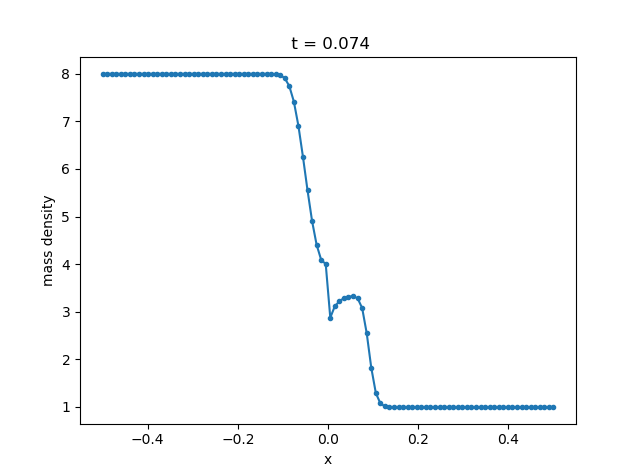
\includegraphics[width=\textwidth]{rs_1}
    \end{subfigure}
    ~ %add desired spacing between images, e. g. ~, \quad, \qquad, \hfill etc. 
      %(or a blank line to force the subfigure onto a new line)
    \begin{subfigure}[b]{0.3\textwidth}
        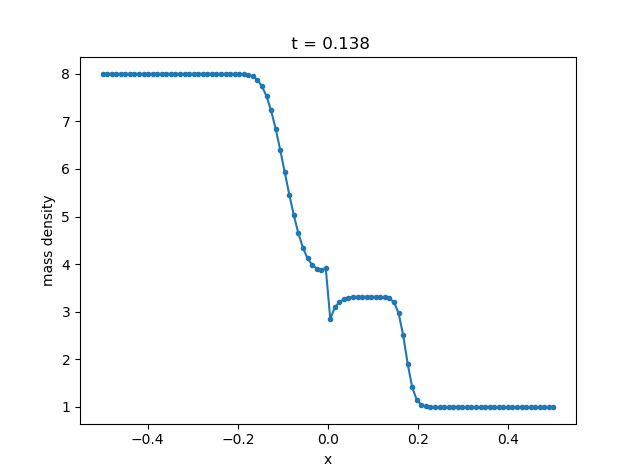
\includegraphics[width=\textwidth]{rs_2}
    \end{subfigure}
    ~ %add desired spacing between images, e. g. ~, \quad, \qquad, \hfill etc. 
    %(or a blank line to force the subfigure onto a new line)
    \begin{subfigure}[b]{0.3\textwidth}
        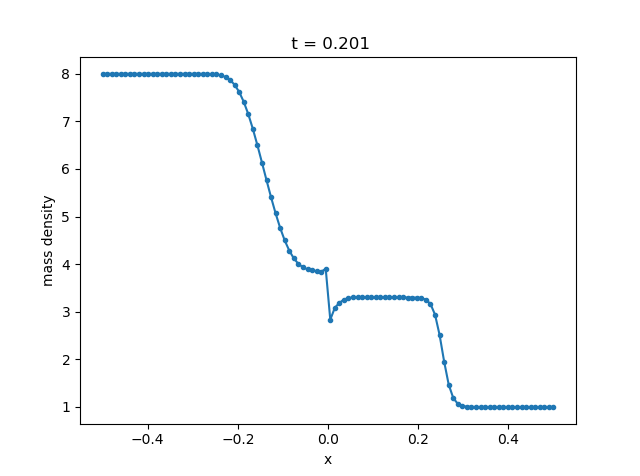
\includegraphics[width=\textwidth]{rs_3}
    \end{subfigure}
    \caption{The mass density at several moments in time for the sod shock problem}\label{fig:rs}
\end{figure}

\begin{figure}[H]
    \centering
    \begin{subfigure}[b]{0.3\textwidth}
        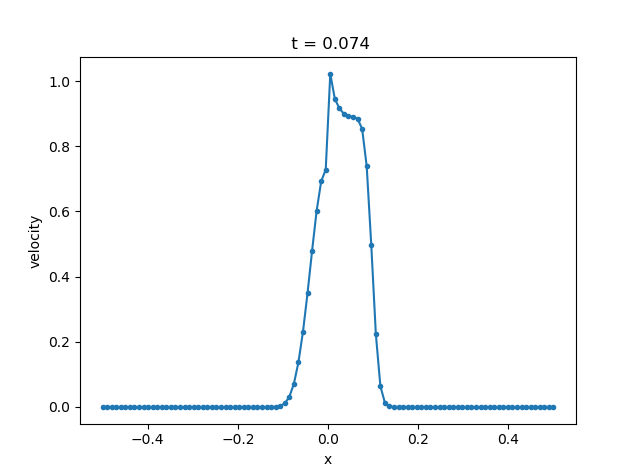
\includegraphics[width=\textwidth]{rvs_1}
    \end{subfigure}
    ~ %add desired spacing between images, e. g. ~, \quad, \qquad, \hfill etc. 
      %(or a blank line to force the subfigure onto a new line)
    \begin{subfigure}[b]{0.3\textwidth}
        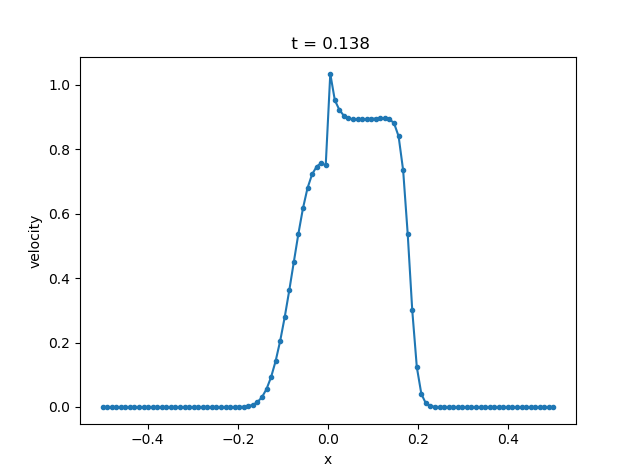
\includegraphics[width=\textwidth]{rvs_2}
    \end{subfigure}
    ~ %add desired spacing between images, e. g. ~, \quad, \qquad, \hfill etc. 
    %(or a blank line to force the subfigure onto a new line)
    \begin{subfigure}[b]{0.3\textwidth}
        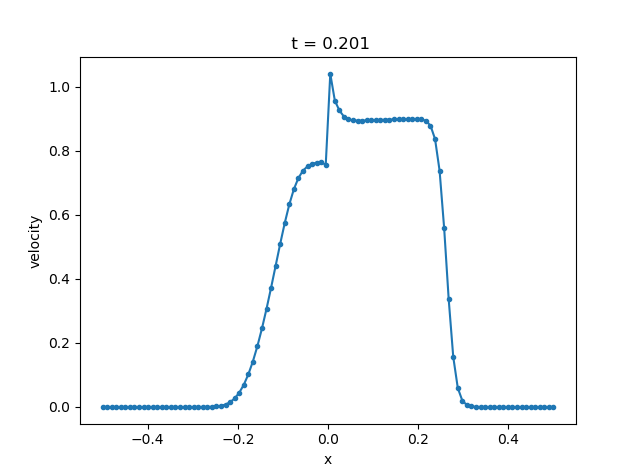
\includegraphics[width=\textwidth]{rvs_3}
    \end{subfigure}
    \caption{The velocity at several moments in time for the sod shock problem}\label{fig:rvs}
\end{figure}

\begin{figure}[H]
    \centering
    \begin{subfigure}[b]{0.3\textwidth}
        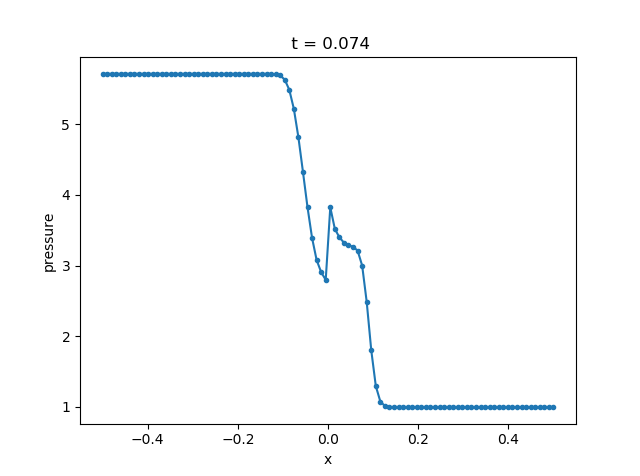
\includegraphics[width=\textwidth]{ps_1}
    \end{subfigure}
    ~ %add desired spacing between images, e. g. ~, \quad, \qquad, \hfill etc. 
      %(or a blank line to force the subfigure onto a new line)
    \begin{subfigure}[b]{0.3\textwidth}
        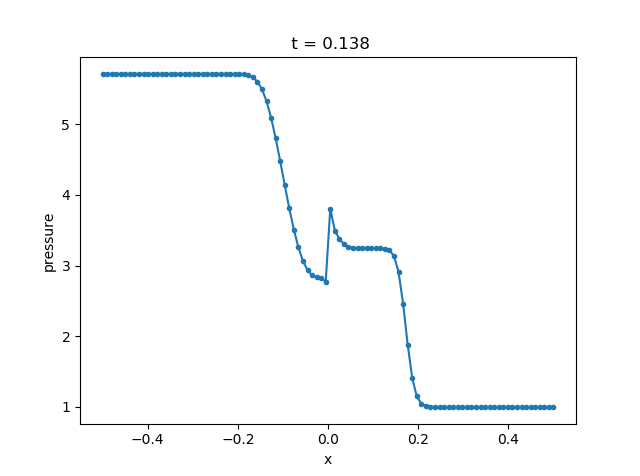
\includegraphics[width=\textwidth]{ps_2}
    \end{subfigure}
    ~ %add desired spacing between images, e. g. ~, \quad, \qquad, \hfill etc. 
    %(or a blank line to force the subfigure onto a new line)
    \begin{subfigure}[b]{0.3\textwidth}
        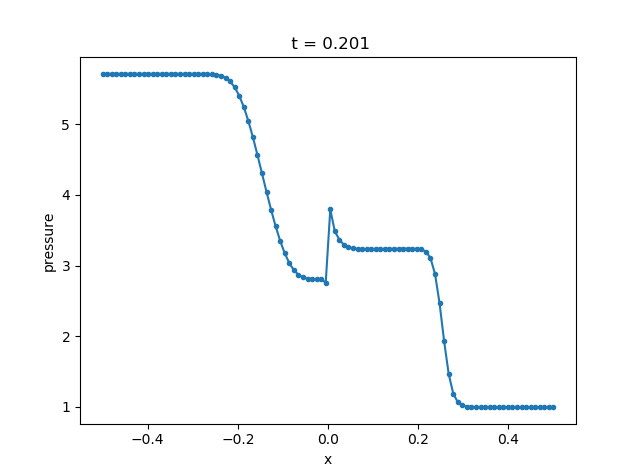
\includegraphics[width=\textwidth]{ps_3}
    \end{subfigure}
    \caption{The pressure at several moments in time for the sod shock problem}\label{fig:ps}
\end{figure}

For each variable you can see three regions appearing. To the left and right there is a region that equals the initial condition, and in the middle we have an intermediate region that expands to the left and right with the wave speeds. 

\subsubsection{Linear acoustic wave problem}
For the linear acoustic wave problem we have a smooth initial condition for $P$ and $\rho$ from $x = 0$ to $x = 1$ and we run the solution up to $t_max = 3$. In the figures \ref{fig:ra}, \ref{fig:rva} and \ref{fig:pa} the profiles of mass density $\rho$, velocity $v$ and pressure $P$ are plotted at several moments in time. 

\begin{figure}[H]
    \centering
    \begin{subfigure}[b]{0.3\textwidth}
        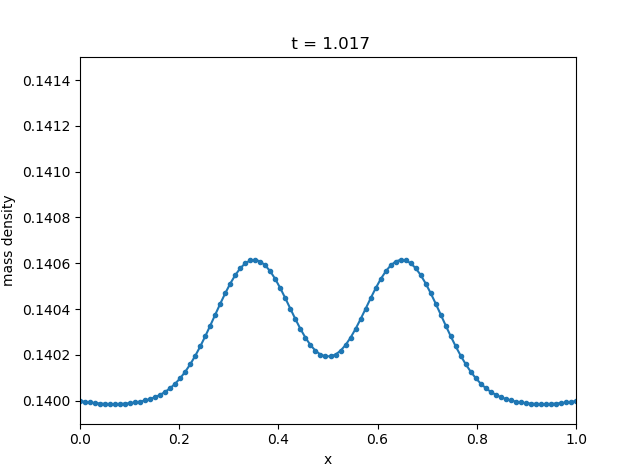
\includegraphics[width=\textwidth]{ra_1}
    \end{subfigure}
    ~ %add desired spacing between images, e. g. ~, \quad, \qquad, \hfill etc. 
      %(or a blank line to force the subfigure onto a new line)
    \begin{subfigure}[b]{0.3\textwidth}
        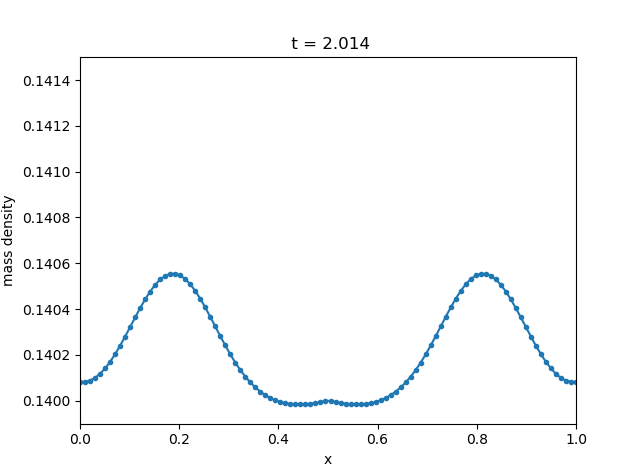
\includegraphics[width=\textwidth]{ra_2}
    \end{subfigure}
    ~ %add desired spacing between images, e. g. ~, \quad, \qquad, \hfill etc. 
    %(or a blank line to force the subfigure onto a new line)
    \begin{subfigure}[b]{0.3\textwidth}
        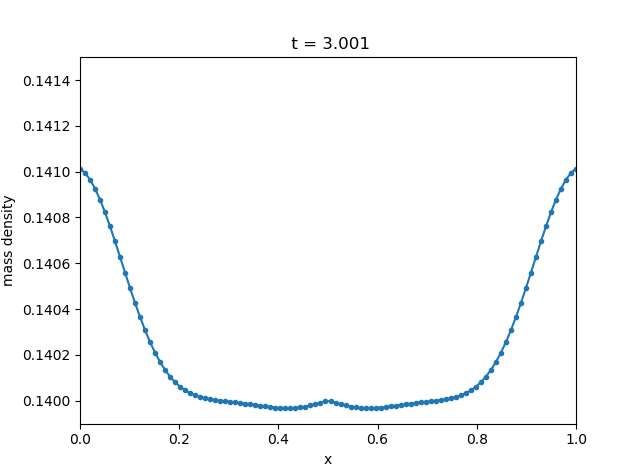
\includegraphics[width=\textwidth]{ra_3}
    \end{subfigure}
    \caption{The mass density at several moments in time for the linear acoustic wave problem}\label{fig:ra}
\end{figure}

\begin{figure}[H]
    \centering
    \begin{subfigure}[b]{0.3\textwidth}
        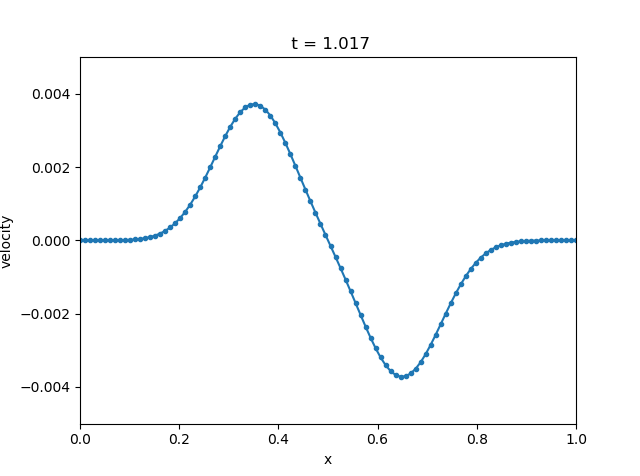
\includegraphics[width=\textwidth]{rva_1}
    \end{subfigure}
    ~ %add desired spacing between images, e. g. ~, \quad, \qquad, \hfill etc. 
      %(or a blank line to force the subfigure onto a new line)
    \begin{subfigure}[b]{0.3\textwidth}
        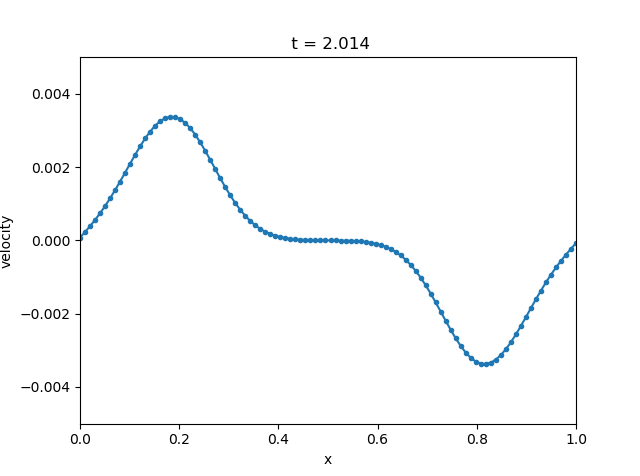
\includegraphics[width=\textwidth]{rva_2}
    \end{subfigure}
    ~ %add desired spacing between images, e. g. ~, \quad, \qquad, \hfill etc. 
    %(or a blank line to force the subfigure onto a new line)
    \begin{subfigure}[b]{0.3\textwidth}
        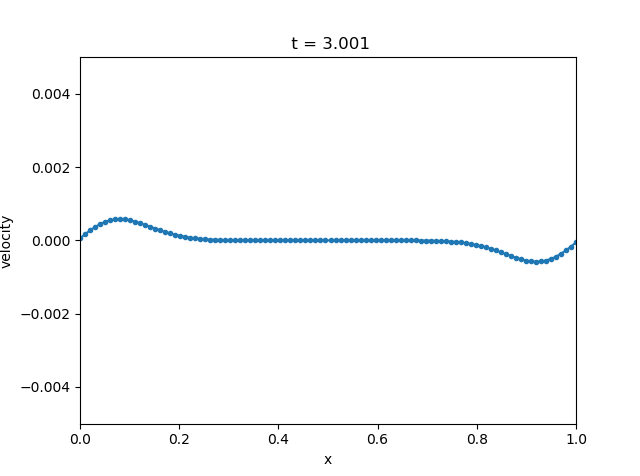
\includegraphics[width=\textwidth]{rva_3}
    \end{subfigure}
    \caption{The velocity at several moments in time for the linear acoustic wave problem}\label{fig:rva}
\end{figure}

\begin{figure}[H]
    \centering
    \begin{subfigure}[]{0.3\textwidth}
        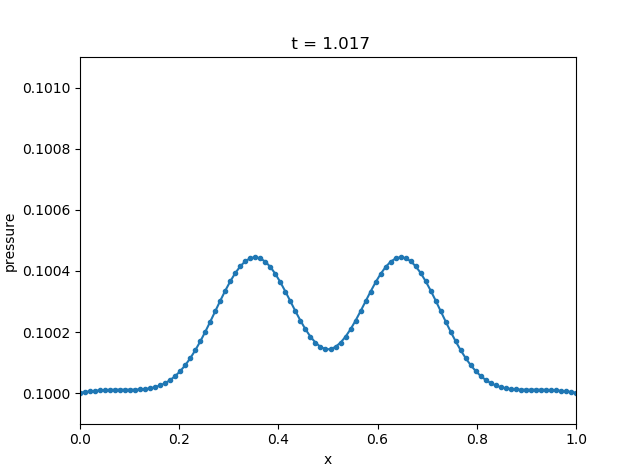
\includegraphics[width=\textwidth]{pa_1}
    \end{subfigure}
    ~ %add desired spacing between images, e. g. ~, \quad, \qquad, \hfill etc. 
      %(or a blank line to force the subfigure onto a new line)
    \begin{subfigure}[]{0.3\textwidth}
        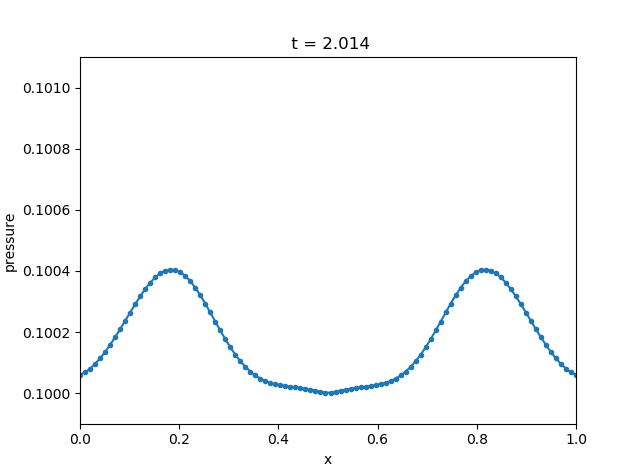
\includegraphics[width=\textwidth]{pa_2}
    \end{subfigure}
    ~ %add desired spacing between images, e. g. ~, \quad, \qquad, \hfill etc. 
    %(or a blank line to force the subfigure onto a new line)
    \begin{subfigure}[]{0.3\textwidth}
        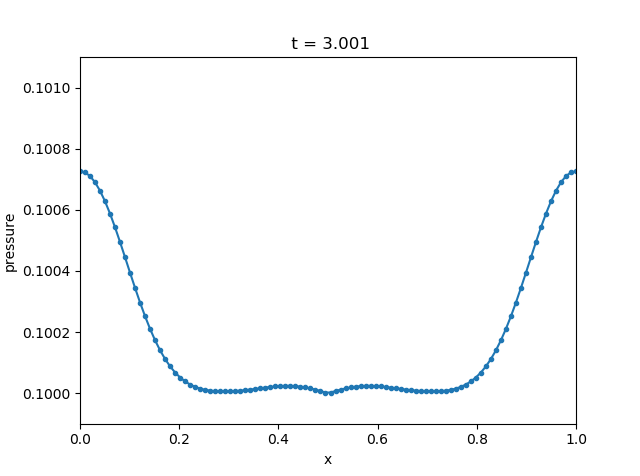
\includegraphics[width=\textwidth]{pa_3}
    \end{subfigure}
    \caption{The pressure at several moments in time for the linear acoustic wave problem}\label{fig:pa}
\end{figure}

As expected, the numerical solution is periodic here \footnote{this is unfortunately not very visible in three images, but can be visualized by plotting several more moments, for which there was no room in this report}.

\subsection{Analysis of the method}
Now that we have our numerical implementation it is important to validate this implementation. Therefore we will study the empirical order of convergence, the dissipation of the method and the total time of computation.

\subsubsection{Computational effort}
For both the sod shock problem and the linear acoustic wave problem we counted the elapsed time between the beginning and the end of the computation. Note that we did not count the computational effort to plot the figures in the elapsed time. 

\begin{table}%
\begin{tabular}{l||c|c}
& sod shock problem & linear acoustic wave problem \\
\hline
\textbf{elapsed time}($s$) & 35.23771614191482 & 213.64273714810716
\end{tabular}
\caption{Computational effort for the sod shock problem and the linear acoustic wave problem on a grid with $nx = 1000$}
\label{time}
\end{table}

As you can see the computational time for the linear acoustic wave problem is larger. That might be because runtime for this problem is larger, namely 3 versus 0.2. 

\subsubsection{Empirical Order of Convergence}
The first order upwind scheme is (as the name suggests), first order accurate in time. By plotting the empirical error of convergence $EOC_nu = \frac{\log\left(\epsilon_{\nu} / \epsilon_{\nu-1}\right)}{\log\left(2^{\nu-1} / 2^{\nu}\right)}$ for $3 \leq nu \leq 12$ we check if this is the case in our implementation. Here $\epsilon_{\nu}$ is the maximum error on a spatial grid $x_i$ for $0 \leq i \leq 2^{\nu}$

Since we only have an analytical solution for the sod shock problem, we used this analytic solution to compute the empirical order of convergence. The results are plotted in figure \ref{EOC}, where we used the mass density as a variable.

\begin{figure}[H]
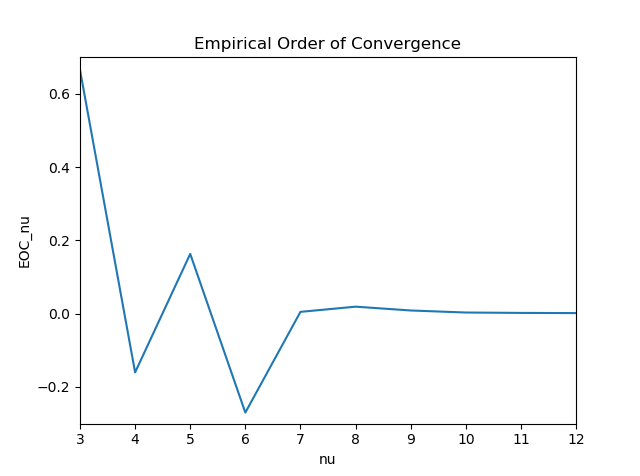
\includegraphics[width=\columnwidth]{eoc}%
\caption{The empirical order of convergence for the maximum error in the mass density of the sod shock problem}%
\label{EOC}%
\end{figure}

In this figure you can see that the empirical error of convergence, tends to 0 when $\nu > 5$ and $nx = 32$. So we can conclude that the order of accuracy for our numerical scheme is 1. 

\subsubsection{Dissipation of the method}
In figure \ref{dissipation} we plotted the analytic and numerical solution for the sod sock problem.

\begin{figure}[H]
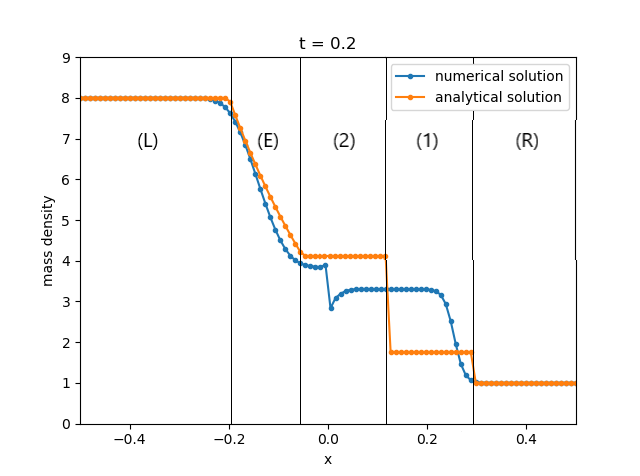
\includegraphics[width=\columnwidth]{dissipation}%
\caption{The analytical and numerical solution for the mass density at time t = 0.02}%
\label{dissipation}%
\end{figure}

In this figure you can clearly see five regions. In regions (R) and (L) the analytical solution and the numerical solution are equal. This is to be expected since this is the initial condition and the shock has not reached these regions yet. In region (E) both the analytical solution and the numerical solution decrease. However the analytical solution decreases linearly and makes a sharp edge with region (L) and (1) whereas the numerical solution makes a much smoother edge with region (L). So here we see dissipation of the numerical scheme. 

Finally in regions (1) and (2) the analytical solution has two distinct values whereas the numerical solution has only one value and some glitches. This could be due to implementation and round-off errors. 

\end{document}